\chapter{Administrateur}

\section{Presentation de l'interface}

\subsection{Acceuil}
 \begin{figure}[H]
 	\centering
 	
 	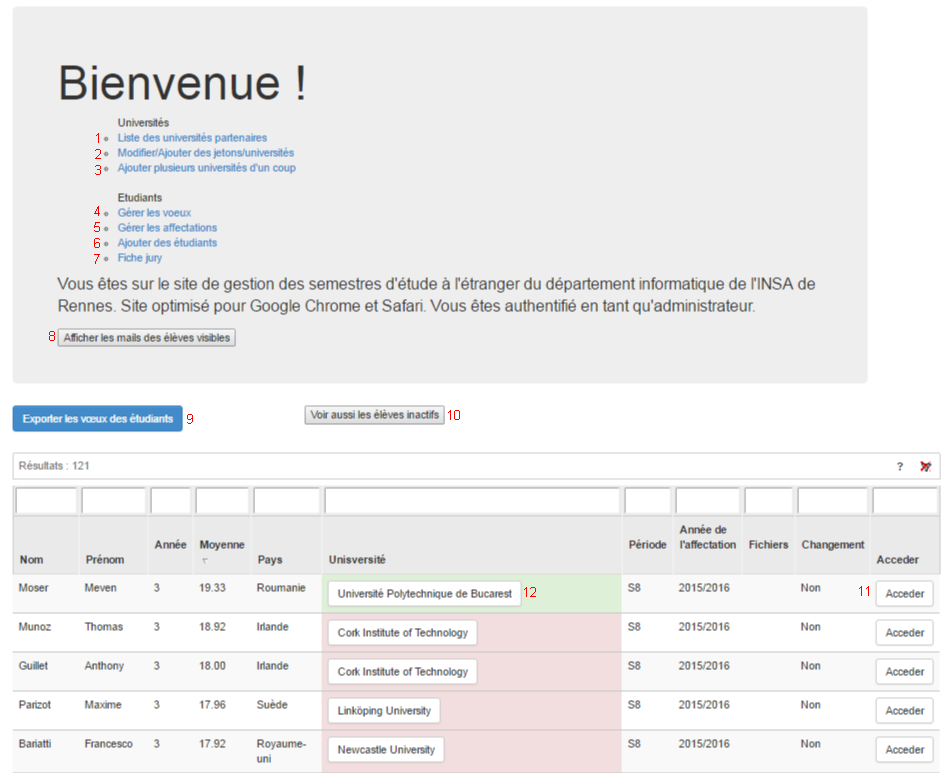
\includegraphics[width=14cm,height=7cm]{Images/Admin/menu_acceuil_admin.png}
 	\caption{Accueil administrateur}
 	\label{aa}
 \end{figure}
 
 
 \subsection{Liste des universités partenaires}
 \begin{figure}[H]
 	\centering
 	
 	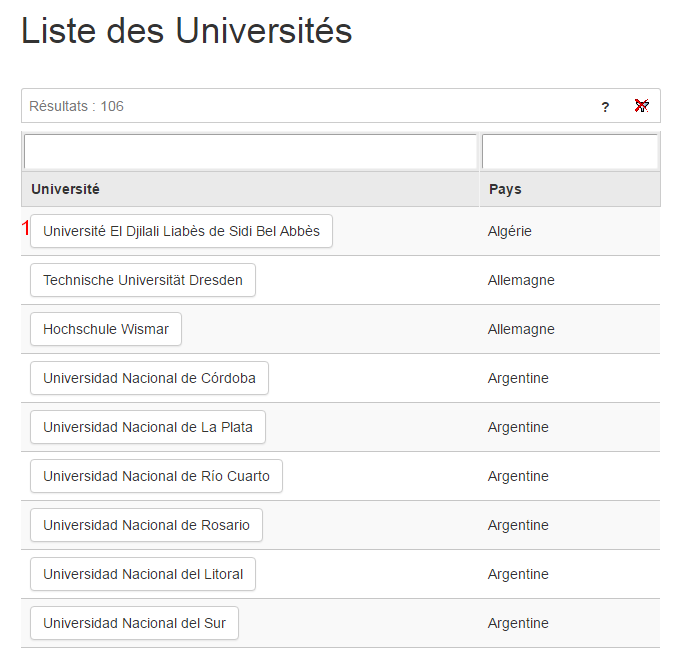
\includegraphics[width=14cm,height=7cm]{Images/Admin/liste_univ_admin.png}
 	\caption{Liste des universités partenaires}
 	\label{lua}
 \end{figure}
 
 
  \subsection{Modifier/Ajouter des jetons/Ajouter des Universités}
  \begin{figure}[H]
  	\centering
  	
  	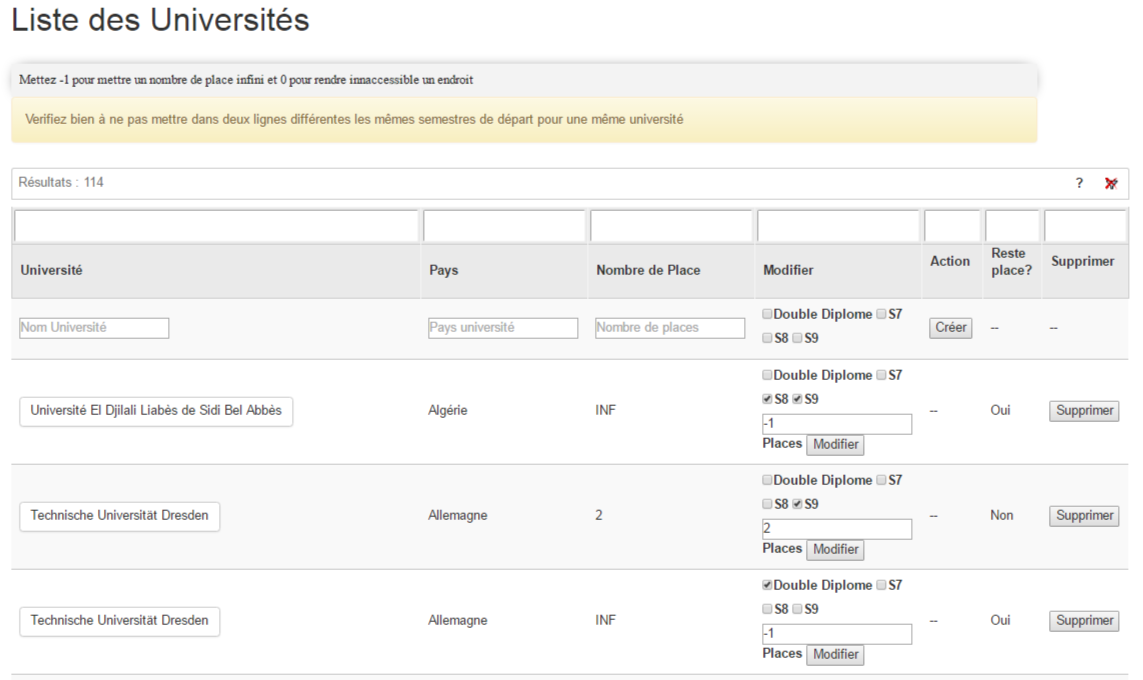
\includegraphics[width=14cm,height=7cm]{Images/Admin/gestion_univ_admin.png}
  	\caption{Modifier/Ajouter des jetons/Ajouter des Universités}
  	\label{gua}
  \end{figure}


  \subsection{Ajouter plusieurs universités}
  \begin{figure}[H]
  	\centering
  	
  	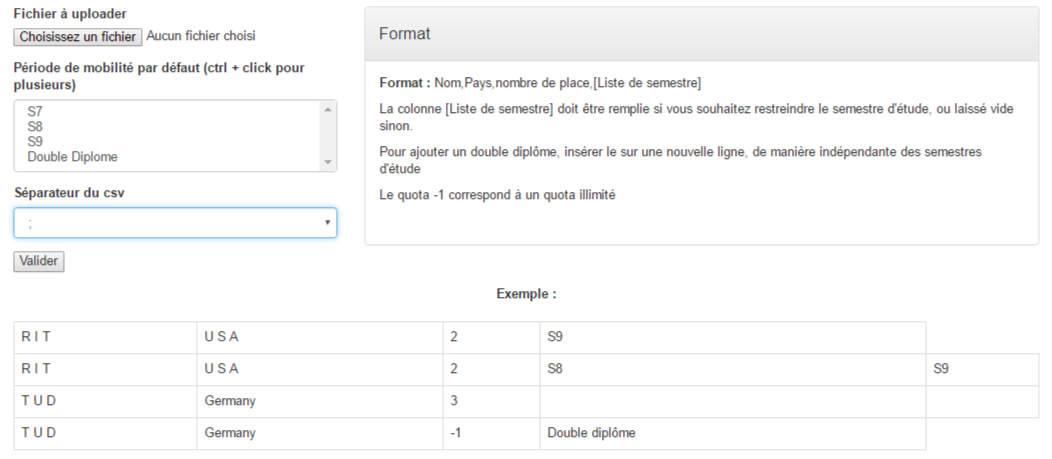
\includegraphics[width=14cm,height=7cm]{Images/Admin/ajout_plusieux_univ_admin.png}
  	\caption{Ajouter plusieurs universités}
  	\label{pua}
  \end{figure}

\section{Gestion des universités}

\subsection{voir la fiche résumé des universités}

Depuis la page d'accueil \ref{aa} cliquez sur le lien "Liste des universités partenaire". Une fois sur cette page, il vous suffit de cliquer sur le nom de l'université de votre choix pour arriver sur sa page personnelle.
 
\subsection{modifier les jetons d'une université : base}

Depuis la page d'accueil \ref{aa} cliquez sur le lien "Modifier/Ajouter des jetons/universités". Vous arrivez sur une page contenant une table avec la liste des universités partenaires. a droite de chaque université, est présente une case "Modifier" dans laquelle vous pouvez modifier la liste des départs disponible à cette destination ainsi que le nombre de place disponible.

\smallbreak

Attention, mettre une valeur de -1 comme nombre de place signifie qu'il y a un nombre illimité de place disponibles.

\subsection{modifier les jetons d'une université : avancé}

Depuis la page de modification des universités (cf paragraphe précédent pour atteindre cette page), si vous souhaitez mettre un nombre de jeton différents pour deux départs différents dans une même université, vous devez créer une nouvelle université ayant le même nom que celle déjà existante puis modifier de manière indépendantes les deux universités.

\subsection{créer une nouvelle université}

Depuis la page de modification des universités (cf paragraphe précédent pour atteindre cette page), dans la première ligne de la table, ajoutez un nom d'université, un pays, un nombre de places disponibles et sélectionnez les types de mobilités puis cliquez sur "créer".

\subsection{ajouter plusieurs universités} 

Depuis la page d'accueil \ref{aa} cliquez sur le lien "Ajoutez plusieurs universités d'un coup". Sur cette page, vous devez uploader un fichier CSV ayant le format décrit dans la case "Format" puis choisir les périodes de mobilités que vous voulez associés à ces universités. Choississez le séparateur correspondant à votre fichier CSV puis cliquer sur valider.

\section{Gestion manuelle des voeux des étudiants}

Depuis la page d'accueil \ref{aa} cliquez sur le lien "Gérer les voeux". Vous arrivez sur une page contenant un tableau résumant par élève la liste de ses 3 premiers voeux. Cliquez ensuite sur "Acceder" pour arriver sur la page élève et pouvoir modifier la liste de ses voeux (ajouter, supprimer) et l'ordre de ses voeux à la place de l'élève (cf section choix des destination du chapitre élève).

\section{Fin de la phase de vœux} 

Depuis la page d'accueil \ref{aa} cliquez sur le lien "Gérer les affectations". Cliquez sur le bouton "Bloquer la possibilité de modifier les veux afin que les élèves ne puissent plus modifier ou ajouter de nouveaux vœux.

\section{Affectation des vœux}

Sur la page de gestion des affectation (cf paragraphe précédent"), une fois la possibilité de faire des vœux bloquée, vous pouvez gérer les affectations. 
////////////////////////////// 

\section{Liste de mails}

Depuis la page d'accueil \ref{aa}, avec les filtres selectionner la liste des étudiants qui vous intéressent puis cliquer sur "Afficher les mails des élèves visibles". Il vous suffit ensuite de copier la liste obtenue dans le champs destinataire de votre logiciel de mail.

\section{Gestion des contrat d'étude}

\subsection{accepter contrat d'étude}
Depuis la page d'accueil, cliquez sur le bouton "acceder" de la ligne correspondant à l'élève souhaité. Un fois sur sa page, si l'élève vous a soumis un contrat d'études, vous pouvez soit le valider en cliquant sur la touche "valider", ou alors le refuser en écrivant si vous le souhaiter une raison à votre refus.

\subsection{rentrer manuellement un contrat d'étude}
Depuis la page d'un élève, vous pouvez ajoutez manuellement un learning agreement et le valider directement.

\section{Dépôt de documents}

Depuis la page d'un étudiant, dans la section "Upload de documents, vous pouvez ajouter des fichiers pour l'élève en question. Pour cela, entrez le nom souhaité pour le document puis cliquer sur "choisissez un fichier" et sélectionnez le fichier. Cliquez enfin sur "envoyer" 

\section{Notes et fiches de jury}

